\documentclass[sans]{beamer}
\usetheme{metropolis}
\usecolortheme{crane}

\usepackage[linesnumbered,ruled,vlined]{algorithm2e} 
\usepackage{lmodern}
\usepackage{tikz}
\usepackage{pdfpages}
\usepackage{listings}
\usepackage{multirow}
\usepackage[utf8]{inputenc}
\usepackage{graphicx}
\usepackage{ulem}
\usetikzlibrary{arrows, positioning, shapes.geometric}
\usetikzlibrary{shadows.blur}
\usetikzlibrary{decorations.pathmorphing}

% hide the footline navigation
\setbeamertemplate{footline}[frame number]{}
\setbeamertemplate{navigation symbols}{}
%\setbeamertemplate{footline}{}

\tikzset{snake it/.style={decorate, decoration=snake}}

\tikzset{
    %Define standard arrow tip
    >=stealth',
}

\tikzset{
    invisible/.style={opacity=0,text opacity=0},
    visible on/.style={alt=#1{}{invisible}},
    alt/.code args={<#1>#2#3}{%
      \alt<#1>{\pgfkeysalso{#2}}{\pgfkeysalso{#3}}
    },
}

\tikzset{
  setstyle/.style={#1},
  %bcg/.default={white},
  setstyle on/.style={alt=#1{}{setstyle}},
}

\tikzset{
  background fill/.style={fill=#1},
  background fill/.default={white},
  fill on/.style={alt=#1{}{background fill}},
}

\tikzset{
  background draw/.style={draw=#1},
  background draw/.default={white},
  draw on/.style={alt=#1{}{background draw}},
}

\tikzset{
  background filldraw/.style 2 args={draw=#1, fill=#2},
  background filldraw/.default={white}{white},
  filldraw on/.style={alt=#1{}{background filldraw}},
}

\tikzset{
  background shade/.style={#1},
  background shade/.default={top color=white, bottom color=white},
  shade on/.style={alt=#1{}{background shade}},
}

\tikzset{
  background shadedraw/.style 2 args={draw=#1, #2},
  background shadedraw/.default={white}{top color=white, bottom color=white},
  shadedraw on/.style={alt=#1{}{background shadedraw}},
}

\definecolor{darkgreen}{rgb}{0.0, 0.6, 0.13}

 \lstset{escapeinside={<@}{@>}, columns=fullflexible, basicstyle=\ttfamily}

 \title{\fontsize{0.905em}{1.5em}\selectfont Symbiotic: finding bugs in C programs}
 \author{
 {Marek~Chalupa}
 }
 \bigskip
 \institute {DevConf 2019 , 25. 1. 2019}
 \date{~\\[1cm]}

\begin{document}

%% -------------------------------------------------------------------
\maketitle
%% -------------------------------------------------------------------

%% -------------------------------------------------------------------
\begin{frame}
\frametitle{Bugs}
\end{frame}
%% -------------------------------------------------------------------


%% -------------------------------------------------------------------
\begin{frame}
\frametitle{Symbolic Execution}
\end{frame}
%% -------------------------------------------------------------------

%% -------------------------------------------------------------------
\begin{frame}[fragile]
\frametitle{Symbolic execution}
\begin{center}
\begin{tabular}{c}
\begin{lstlisting}[language=C]
int a = *, b = *, c = *;

if (a > 0) {
  c = 2;
  if (b < 0) {
    c = b
  }
} else {
    c = -2;
}
if (a + b + c <= 0)
  error();
\end{lstlisting}
\end{tabular}
\end{center}
\end{frame}
%% -------------------------------------------------------------------

%% -------------------------------------------------------------------
\begin{frame}[fragile]
\frametitle{Symbolic execution}
\begin{center}
\begin{tikzpicture}[
  scale=1.0,
  sibling distance=10em,
  every node/.style = {scale=1.13, shape=rectangle,
                       align=center, font=\small},
  nd/.style = {draw, font=\ttfamily\tiny,fill=white},
  cond/.style = {font=\tiny, fill=white, text=blue},
  mem/.style = {overlay, font=\tiny} ]
  \node [nd] (root) {if (a > 0);}
    child { node [nd,xshift=-4mm] {c = -2}
      child { node [nd,yshift=-14.5mm] {if (a + b + c <= 0);}
        child { node [nd] {error()}
            edge from parent node[cond,yshift=-.6mm] {$[\alpha + \beta -2 > 0]$}
        }
        child { node [nd] {}
            edge from parent node[cond] {$[\alpha + \beta -2 \le 0]$}
        }
      }
      edge from parent node[cond] {$[\alpha \le 0]$}
    }
    child { node [nd,xshift=4mm] {c = 2}
     child { node [nd, yshift=8mm]  {b < 0;}
       child { node [nd, xshift=8mm] {if (a + b + c <= 0);}
         child { node [nd] {error();}
           %edge from parent node[cond] {$[\alpha + \beta + 2 > 0]$}
         }
         edge from parent node[cond] {$[\beta \ge 0]$}
       }
       child { node [nd] {c = b;}
         child { node [nd] { if (a + b + c <= 0);}
           child { node [nd] { error();}
             edge from parent node[cond,yshift=-.5mm] {$[\alpha + \beta + \beta > 0]$}
           }
           child { node [nd] {}
             edge from parent node[cond] {$[\alpha + \beta + \beta \le 0]$}
           }
         }
         edge from parent node[cond] {$[\beta < 0]$}
       }
    }
    edge from parent node[cond] {$[\alpha > 0]$}
   }
   ;
  \node[mem, scale=1.15, yshift=.5cm, xshift=-3cm] {a := $\alpha$, b := $\beta$, c := $\gamma$};
\end{tikzpicture}
\end{center}
\end{frame}
%% -------------------------------------------------------------------

%% -------------------------------------------------------------------
\begin{frame}
\frametitle{KLEE}
\begin{itemize}
  \item Open-source symbolic executor.
  \item \url{http://klee.github.io/}
\end{itemize}
\bigskip
\begin{center}

\includegraphics[width=4cm]{klee.png}
\end{center}
\end{frame}
%% -------------------------------------------------------------------

%% -------------------------------------------------------------------
\begin{frame}[fragile]
\frametitle{KLEE}
\begin{center}
\begin{tikzpicture}[
    fl/.style = {overlay, draw, font=\ttfamily\tiny,fill=white,
                 minimum height=1cm, minimum width=0.7cm},
  ]
  \node[fl] (source1) at (.8,  2.3) {.c};
  \node[fl] (source2) at (1,2.2) {.c};
  \node[fl] (source3) at (1.2,2.1) {.c};
  \node[overlay] (sources) at (1,1.5) {};
  %\node[overlay,font=\itshape] (sources) at (1,1) {sources};
  \node[fl] (test1) at (9.8 ,-2) {test};
  \node[fl] (test2) at (10  ,-2.2) {test};
  \node[fl] (test3) at (10.2,-2.4) {test};
  \node[overlay] (tests) at (10,-1.5) {};
  \node[] (llvm) at (1,0) {LLVM};
  \node[] (klee) at (10, 0) {KLEE};
  \draw[->] (llvm) -> (klee);
  \draw[->] (sources) edge (llvm);
  \draw[->] (klee) edge (tests);
\end{tikzpicture}
\end{center}
\end{frame}
%% -------------------------------------------------------------------

%% -------------------------------------------------------------------
\begin{frame}[fragile]
\frametitle{Symbiotic}
\begin{center}
\begin{tikzpicture}[
    fl/.style = {overlay, draw, font=\ttfamily\tiny,fill=white,
                 minimum height=1cm, minimum width=0.7cm},
    bullet/.style = {overlay, draw, fill=black,
                     %minimum height=.1cm, minimum width=.1cm,
                     circle, outer sep=.5em},
  ]
  \node[fl] (source1) at (-.2, 2.3) {.c};
  \node[fl] (source2) at (0,  2.2) {.c};
  \node[fl] (source3) at (0.2,2.1) {.c};
  \node[overlay] (sources) at (0,1.5) {};
  %\node[overlay,font=\itshape] (sources) at (1,1) {sources};
  \node[fl] (test1) at (9.8 ,-2) {test};
  \node[fl] (test2) at (10  ,-2.2) {test};
  \node[fl] (test3) at (10.2,-2.4) {test};
  \node[overlay] (tests) at (10,-1.5) {};
  \node[] (llvm) at (0,0) {LLVM};
  \node[] (klee) at (10, 0) {KLEE};
  \draw[->] (llvm) -> (klee);
  \draw[->] (sources) edge (llvm);
  \draw[->] (klee) edge (tests);

  \node[bullet] (opt1-bullet) at (2.5,0) {};
  \node[overlay] (opt1) at (2.5,-2) {optimizations};
  \draw[->, dashed,overlay] (opt1) -> (opt1-bullet);

  \node[bullet] (slicing-bullet) at (5,0) {};
  \node[overlay] (slicing) at (5,2) {slicing};
  \draw[->, dashed,overlay] (slicing) -> (slicing-bullet);

  \node[bullet] (opt2-bullet) at (7.5,0) {};
  \node[overlay] (opt2) at (7.5,-2) {optimizations};
  \draw[->, dashed,overlay] (opt2) -> (opt2-bullet);
\end{tikzpicture}
\end{center}
\end{frame}
%% -------------------------------------------------------------------


\end{document}
